\newpage
\section{Auswertung}
\label{sec:Auswertung}
In diesem Abschnitt werden die aufgenommenen Messdaten in Grafiken sowie Tabellen dargestellt und ausgewertet. Grafiken sowie dazugehörige Rechnungen sind mit Python \cite{python} erstellt bzw. berechnet worden.

\subsection{Messung des Magnetfeldes}
\label{sec:magFeld}
Als erstes wird das Magnetfeld am Ort der Probe bestimmt, dazu werden die Messdaten aus Tabelle \ref{tab:magFeld} in Abbildung \ref{abb:magFeld} visualisiert. Dafür wird die Magnetfeldstärke gegen den Ort aufgetragen.
Der maximale Wert $B_\mathrm{max}$ mit dem die weiteren Rechnungen durchgeführt werden ist gegeben durch:
\begin{equation}
  B_\mathrm{max}=\SI{409}{\milli\tesla}
\end{equation}
Dieser legt damit das Magnetfeld am Ort $Z$ der Probe fest.
\begin{figure}[h!]
  \centering
  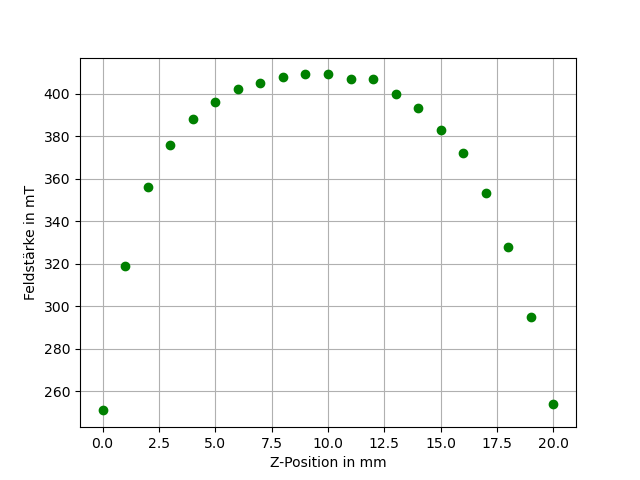
\includegraphics[scale=0.7]{fig/bfeld.png}
  \caption{Zusammenhang zwischen Magnetfeldstärke und Ort im Magnetfeld.}
  \label{abb:magFeld}
\end{figure}
\FloatBarrier

\begin{table}[h!]
  \centering
  \caption{Messdaten der Messung mit der Hallsonde.}
  \label{tab:magFeld}
  \begin{tabular}{c | c}
    \toprule
    Position in $\SI{}{\milli\meter}$ & Magnetfeldstärke in $\SI{}{\milli\tesla}$ \\
    \midrule
    0.0 & 251.0 \\
    1.0 & 319.0 \\
    2.0 & 356.0 \\
    3.0 & 376.0 \\
    4.0 & 388.0 \\
    5.0 & 396.0 \\
    6.0 & 402.0 \\
    7.0 & 405.0 \\
    8.0 & 408.0 \\
    9.0 & 409.0 \\
    10.0 & 409.0 \\
    11.0 & 407.0 \\
    12.0 & 407.0 \\
    13.0 & 400.0 \\
    14.0 & 393.0 \\
    15.0 & 383.0 \\
    16.0 & 372.0 \\
    17.0 & 353.0 \\
    18.0 & 328.0 \\
    19.0 & 295.0 \\
    20.0 & 254.0 \\
    \bottomrule
  \end{tabular}
\end{table}
\FloatBarrier
\newpage
\subsection{Messung mit undotiertem Galliumarsenid}
\label{sec:undotiert}
In diesem Auswertungsabschnitt wird die undotierte Galliumarsenid-Probe betrachtet.
Mit der Dicke der Probe $L_\mathrm{undotiert}=\SI{5.11}{\milli\meter}$ und den gemessenen Werten wird ein normierter Wert der Faradayrotation bestimmt. Dazu wird zunächst die Formel (\ref{eqn:rotawinkel}) benutzt um den Differenzwinkel $\vartheta$ zu bestimmen, anschließend
wird dieser Wert in [$\SI{}{\radian\per\milli\meter}$] umgerechnet. Mit Hilfe von Gleichung (\ref{eqn:umrechnung}) wird der normierte Wert $\vartheta_\mathrm{norm}$ erhalten. Die Formel für die Umrechnung lautet:
\begin{equation}
  \label{eqn:umrechnung}
  \vartheta_\mathrm{norm}=\dfrac{2\pi}{360}\dfrac{\vartheta}{L_\mathrm{undotiert}}
\end{equation}
In der Tabelle \ref{tab:undot} sind die Messdaten für die verschiedenen Wellenlängen $\lambda$ sowie den dazugehörigen Winkeln $\vartheta_\mathrm{+B}$ und $\vartheta_\mathrm{-B}$, als auch den normierten Rotationswinkel $\vartheta_\mathrm{norm}$ zu finden.
In Abbildung \ref{abb:undot} sind die normierten Rotationswinkel $\vartheta_\mathrm{norm}$ gegen die Quadrate der Wellenlängen $\lambda^2$ aufgetragen.
\begin{table}
  \centering
  \caption{Messdaten der undotierten Galliumarsenid-Probe und normierte Rotationswinkel in $\SI{}{\radian\per\milli\meter}$.}
  \label{tab:undot}
  \begin{tabular}{c | c | c | c}
    \toprule
    $\lambda$/$\SI{}{\micro\meter}$ & $\vartheta_\mathrm{+B}$/$\SI{}{\degree}$ & $\vartheta_\mathrm{-B}$/$\SI{}{\degree}$& $\vartheta_{\mathrm{norm}}$/$\SI{}{\radian\per\milli\meter}$ \\
    \midrule
    1.06 & 267.0 & 243.0 & 0.082 \\
    1.29 & 261.0 & 248.5 & 0.043 \\
    1.45 & 261.2 & 250.0 & 0.038 \\
    1.72 & 258.0 & 249.9 & 0.028 \\
    1.96 & 252.0 & 244.8 & 0.025 \\
    2.156 & 248.7 & 243.5 & 0.018 \\
    2.34 & 225.6 & 221.5 & 0.014 \\
    2.51 & 212.0 & 208.4 & 0.012 \\
    2.65 & 177.0 & 173.4 & 0.012 \\
    \bottomrule
  \end{tabular}
\end{table}
\FloatBarrier

\begin{figure}
  \centering
  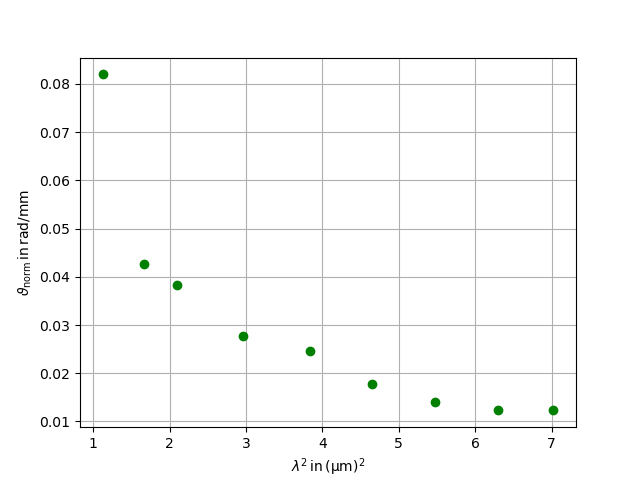
\includegraphics[scale=0.7]{fig/undotiert.png}
  \caption{Grafische Darstellung der Messdaten der undotierten Probe.}
  \label{abb:undot}
\end{figure}
\FloatBarrier

\subsection{Messung mit dotierten Galliumarsenid-Proben}
\label{sec:dot}
In dieser Messung werden nun die dotierten Galliumarsenid-Proben verwendet.
Die zu untersuchenden Proben haben jeweils die Dicken $L_{\mathrm{leicht}}=\SI{1.296}{\milli\meter}$ bzw. $L_{\mathrm{hoch}}=\SI{1.36}{\milli\meter}$ und eine Donatorenkonzentration von $N_{\mathrm{leicht}}=\SI{1.2 e18}{\per\centi\cubic\meter}$ bzw. $N_{\mathrm{hoch}}=\SI{2.8 e18}{\per\centi\cubic\meter}$.
In den Tabellen \ref{tab:tief} und \ref{tab:hoch} sind die erhaltenen Messdaten aufgelistet, die normierten Rotationsinkel werden wieder mit Gleichung (\ref{eqn:umrechnung}) berechnet, allerdings jeweils mit den Längen $L_{\mathrm{leicht}}$ bzw. $L_{\mathrm{hoch}}$:
Von den erhaltenen Werten werden für alle Wellenlängen die normierte Faradayrotation der undotierten Probe abgezogen.
So kann die differenzierte Faradayrotation $\Delta\vartheta_\mathrm{norm}$, die durch Leitungselektronen bedingt ist, untersucht werden.
Die berechneten Werte sind in Abbildung \ref{abb:delta} grafisch dargestellt..
Bei der leicht dotierten Probe fällt ein Wert weit aus der Reihe und wird nicht für die lineare Ausgleichrechnung berücksichtigt.
Die Daten werden mit der folgenden Funktion gefittet
\begin{equation}
  \Delta\vartheta_{\mathrm{norm}} = A\lambda^2
\end{equation}
Daraus ergeben sich für die beiden Proben die Parameter:
\begin{align*}
  A_{\mathrm{leicht}} &= \SI{0.0170526 \pm 0.0000031}{\radian\per\nano\cubic\meter} \\
  A_{\mathrm{hoch}} &= \SI{0.0283207 \pm 0.0000036}{\radian\per\nano\cubic\meter}
\end{align*}
Mit Hilfe der Gleichung (\ref{eqn:massewinkel}) und den jeweiligen Parametern $A_{\mathrm{leicht}}$ bzw. $A_{\mathrm{hoch}}$ ist es nun möglich die effektive Masse zu bestimmen.
Für den Brechungsindex von Galliumarsenid wird $n \approx 3.4$ \cite{nGaAs} genutzt.
Mit der Formel:
\begin{equation}
  m^*=\sqrt{\frac{e^3\cdot N \cdot B}{A\cdot 8\pi^2\varepsilon_\mathrm{0} c^3 \cdot n }}
\end{equation}
ergeben sich die für die effektive Masse mit $m_\mathrm{e} = \SI{9.10938356 e-31}{\kilogram}$ als Elektronenmasse folgende Werte:
\begin{align*}
  m^*_{\mathrm{leicht}} &= \SI{4.2992 \pm 0.0004 e-32}{\kilogram} \\
  \frac{m^*_{\mathrm{leicht}}}{m_\mathrm{e}} &= 0.047195\pm 0.000004 \\
  m^*_{\mathrm{hoch}} &= \SI{5.09582 \pm 0.00032 e-32}{\kilogram} \\
  \frac{m^*_{\mathrm{hoch}}}{m_\mathrm{e}} &= 0.055940\pm 0.000004\\
\end{align*}

\begin{table}[h!]
  \centering
  \caption{Messdaten der leicht dotierten Galliumarsenid-Probe und normierte Rotationswinkel in $\SI{}{\radian\per\milli\meter}$.}
  \label{tab:tief}
  \begin{tabular}{c | c | c | c}
    \toprule
    $\lambda$/$\SI{}{\micro\meter}$ & $\vartheta_\mathrm{+B}$/$\SI{}{\degree}$ & $\vartheta_\mathrm{-B}$/$\SI{}{\degree}$& $\vartheta_{\mathrm{norm}}$/$\SI{}{\radian\per\milli\meter}$ \\
    \midrule
    1.06 & 260.0 & 251.9 & 0.022 \\
    1.29 & 259.0 & 251.0 & 0.060 \\
    1.45 & 258.7 & 252.5 & 0.041 \\
    1.72 & 257.0 & 250.0 & 0.062 \\
    1.96 & 252.0 & 244.3 & 0.074 \\
    2.156 & 250.1 & 240.7 & 0.103 \\
    2.34 & 227.3 & 219.1 & 0.091 \\
    2.51 & 206.9 & 206.0 & -0.001 \\
    2.65 & 242.7 & 235.0 & 0.087 \\
    \bottomrule
  \end{tabular}
\end{table}

\begin{table}[h!]
  \centering
  \caption{Messdaten der hoch dotierten Galliumarsenid-Probe und normierte Rotationswinkel in $\SI{}{\radian\per\milli\meter}$.}
  \label{tab:hoch}
  \begin{tabular}{c | c | c | c}
    \toprule
    $\lambda$/$\SI{}{\micro\meter}$ & $\vartheta_\mathrm{+B}$/$\SI{}{\degree}$ & $\vartheta_\mathrm{-B}$/$\SI{}{\degree}$& $\vartheta_{\mathrm{norm}}$/$\SI{}{\radian\per\milli\meter}$ \\
    \midrule
    1.06 & 260.0 & 251.9 & 0.022 \\
    1.29 & 259.0 & 251.0 & 0.060 \\
    1.45 & 258.7 & 252.5 & 0.041 \\
    1.72 & 257.0 & 250.0 & 0.062 \\
    1.96 & 252.0 & 244.3 & 0.074 \\
    2.156 & 250.1 & 240.7 & 0.103 \\
    2.34 & 227.3 & 219.1 & 0.091 \\
    2.51 & 206.9 & 206.0 & -0.001 \\
    2.65 & 242.7 & 235.0 & 0.087 \\
    \bottomrule
  \end{tabular}
\end{table}

\begin{figure}[h!]
  \centering
  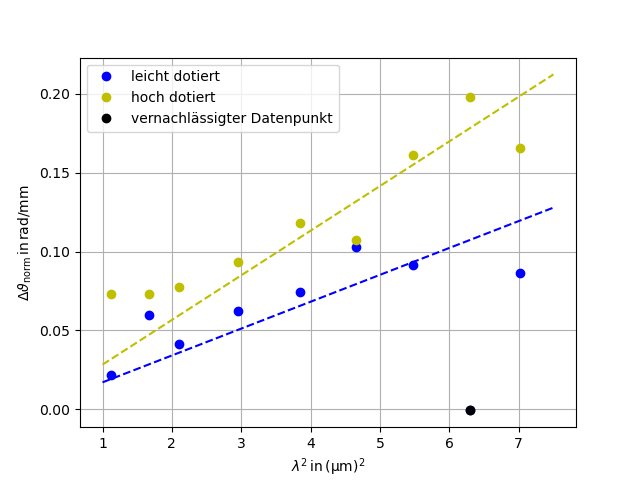
\includegraphics[scale=0.7]{fig/deltaTheta.png}
  \caption{Grafische Darstellung der Messdaten aus den Tabellen \ref{tab:tief} und \ref{tab:hoch}.}
  \label{abb:delta}
\end{figure}
